% NetMob 2026 poster, A0 portrait (841 x 1189 mm). pdfLaTeX.
\documentclass{article}
\usepackage[paperwidth=841mm,paperheight=1189mm,margin=0mm]{geometry}
\usepackage[T1]{fontenc}
\usepackage{lmodern}
\usepackage{tgheros}
\renewcommand{\familydefault}{\sfdefault}
\usepackage{xcolor}
\usepackage{tikz}
\usetikzlibrary{positioning,calc,fit,decorations.pathreplacing}
\usepackage{pgfplots}
\pgfplotsset{compat=1.17}
\usepackage{amsmath}
\usepackage{booktabs}
\usepackage{tabularx}
\usepackage{enumitem}
\usepackage{qrcode}
\pagestyle{empty}
\pdfminorversion=4
\pdfinfo{
  /Title (BUBBLE-BLUE: private group messaging over an open Bluetooth LE mesh)
  /Author (Paul-Maxence Baraton, Nadjib Achir, Philippe Jacquet, Wilfred Dore)
  /Subject (NetMob 2026 poster, A0 portrait 841 x 1189 mm, print-ready)
  /Keywords (BUBBLE-BLUE, NetMob 2026, Bluetooth mesh)
}
\setlength{\parindent}{0pt}
\setlength{\parskip}{5mm}

\definecolor{navy}{HTML}{14213D}
\definecolor{accent}{HTML}{C8102E}
\definecolor{ink}{HTML}{1F2937}
\definecolor{muted}{HTML}{5B6472}
\definecolor{scr}{HTML}{DCE6F5}
\definecolor{rel}{HTML}{DCEFE3}
\definecolor{hdr}{HTML}{EEF0F3}
\definecolor{newk}{HTML}{FCE9C8}

\newcommand{\body}{\fontsize{29}{38}\selectfont}
\renewcommand{\small}{\fontsize{24}{31}\selectfont}
\newcommand{\sect}[1]{\par\vfill\vspace{8mm}%
  {\color{navy}\fontsize{46}{52}\selectfont\bfseries #1\par}%
  \vspace{2mm}{\color{accent}\rule{\linewidth}{1.2mm}}\par\vspace{2mm}}
\newcommand{\firstsect}[1]{%
  {\color{navy}\fontsize{46}{52}\selectfont\bfseries #1\par}%
  \vspace{2mm}{\color{accent}\rule{\linewidth}{1.2mm}}\par\vspace{2mm}}
\newcommand{\fig}[1]{\par\vspace{1mm}{\small\color{muted}#1\par}}
\setlist{nosep, leftmargin=9mm, itemsep=2mm, label=\textbullet}
\setlength{\tabcolsep}{4mm}
\renewcommand{\arraystretch}{1.25}

\pgfplotsset{every axis/.append style={
  font=\small, width=0.93\linewidth, height=95mm, scale only axis=false,
  grid=major, grid style={gray!25}, axis line style={muted},
  tick style={muted}, label style={font=\small}, tick label style={font=\small},
  legend style={font=\small, draw=none, fill=white, fill opacity=0.85, text opacity=1}}}

\begin{document}
\color{ink}
\begin{tikzpicture}[remember picture, overlay]
  \fill[navy] (current page.north west) rectangle ([yshift=-165mm]current page.north east);
  \fill[accent] ([yshift=-165mm]current page.north west) rectangle ([yshift=-168mm]current page.north east);
\end{tikzpicture}

% ---------------------------------------------------------------- header
\vspace*{24mm}
\hspace*{32mm}\begin{minipage}[t]{640mm}
  {\color{white}\fontsize{78}{86}\selectfont\bfseries BUBBLE-BLUE: private group messaging\\[2mm]
   over an open Bluetooth LE mesh\par}
  \vspace{9mm}
  {\color{white}\fontsize{32}{40}\selectfont Paul-Maxence Baraton$^1$, Nadjib Achir$^1$,
   Philippe Jacquet$^1$, Wilfred Doré$^2$\par}
  \vspace{3mm}
  {\color{white!80!navy}\fontsize{25}{32}\selectfont $^1$Inria, France \qquad $^2$Qualcomm, France
   \qquad paul-maxence.baraton@inria.fr\par}
\end{minipage}\hfill
\begin{minipage}[t]{110mm}
  \vspace{-2mm}\centering
  \colorbox{white}{\qrcode[height=78mm]{https://arxiv.org/abs/2509.00967}}\\[2mm]
  {\color{white!80!navy}\fontsize{19}{23}\selectfont arXiv:2509.00967}
\end{minipage}\hspace*{32mm}

\vspace{46mm}
\body
\hspace*{30mm}%
% ================================================================ column 1
\begin{minipage}[t][935mm][t]{245mm}
\firstsect{1\enspace The idea}
Where infrastructure is absent, saturated or not trusted (a crowd, a
disaster site, an event), devices can still reach each other over
Bluetooth. Existing Bluetooth meshes either require provisioning, so a
stranger cannot relay, or let every relay read every message [2--4].
BUBBLE-BLUE separates two things:
\begin{itemize}
  \item the \textbf{mesh} is open: any board may join and relay,
        including traffic it cannot decrypt, and nobody pairs;
  \item a \textbf{bubble} is a group defined by a key: only its members
        read its messages.
\end{itemize}

\sect{2\enspace How a message travels}
\begin{center}
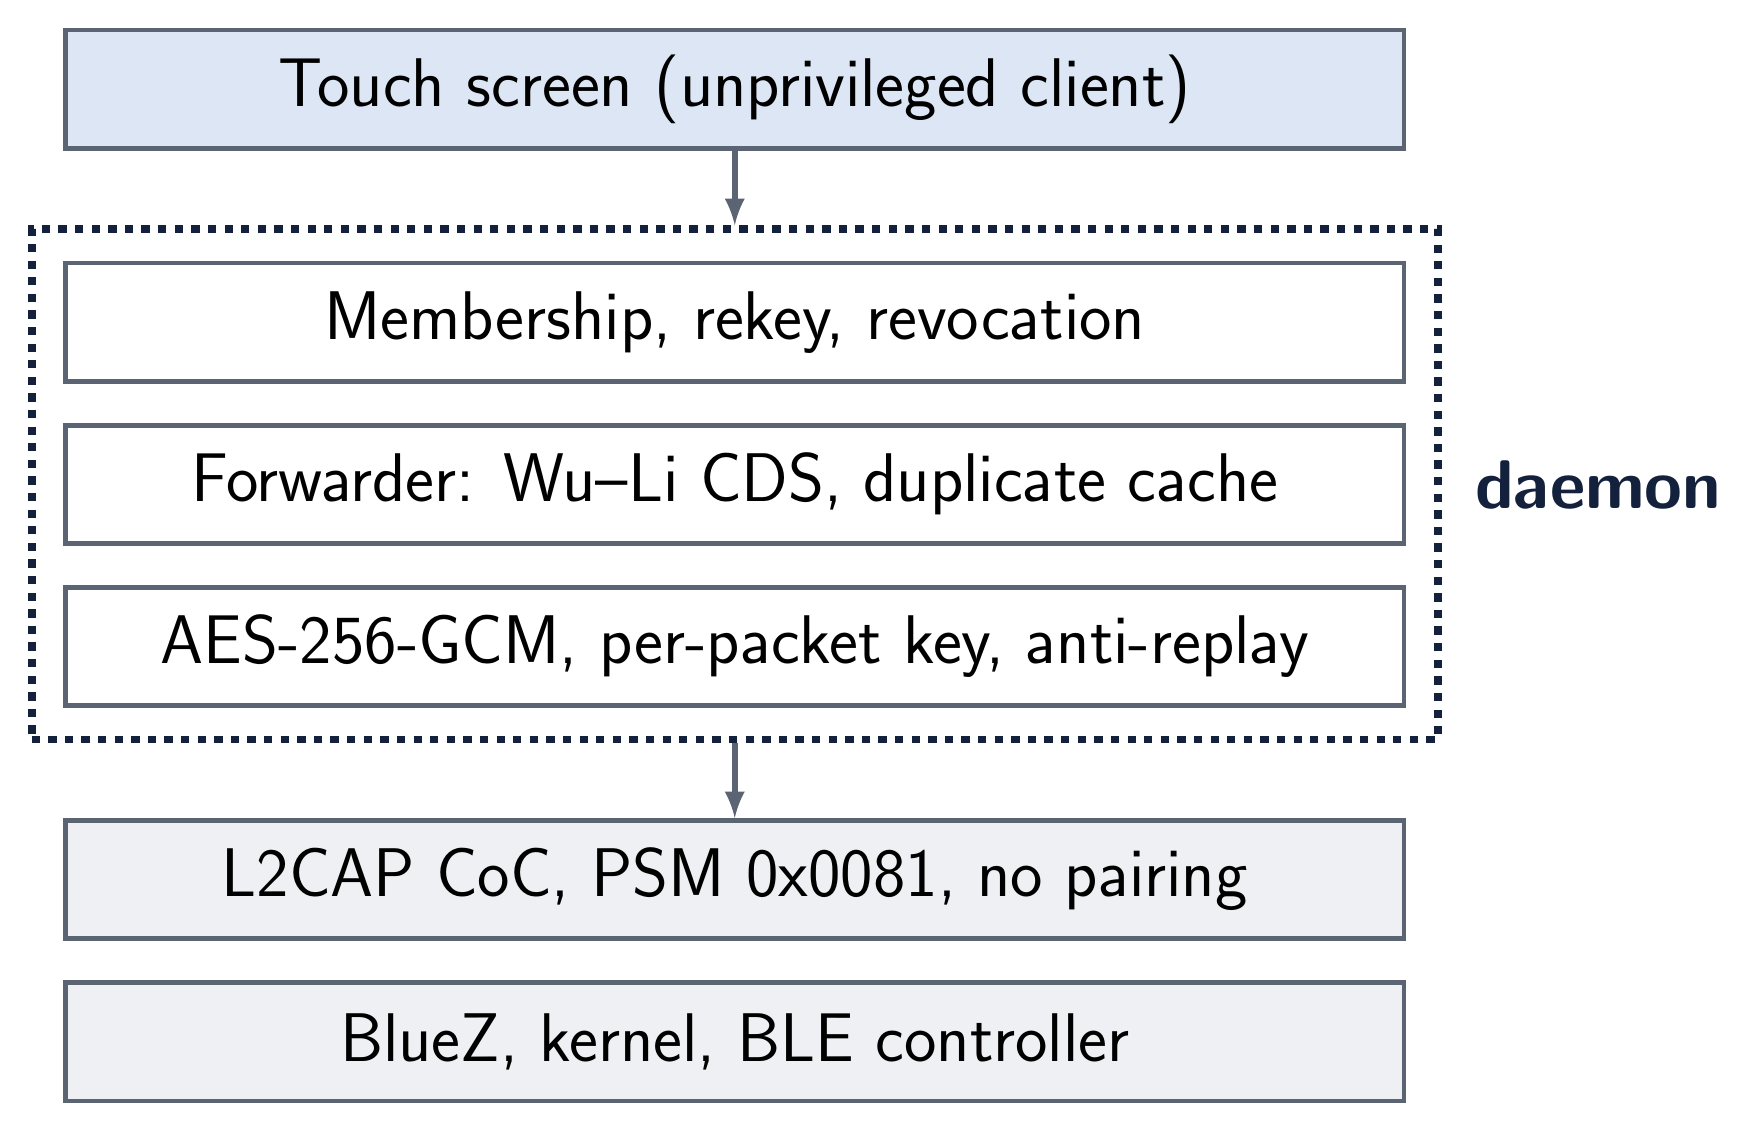
\begin{tikzpicture}[font=\small, node distance=5mm,
  b/.style={draw=muted, fill=#1, minimum width=170mm, minimum height=15mm, align=center, line width=0.6mm},
  b/.default=white]
  \node[b=scr] (ui) {Touch screen (unprivileged client)};
  \node[b, below=14mm of ui] (mem) {Membership, rekey, revocation};
  \node[b, below=of mem] (fwd) {Forwarder: Wu--Li CDS, duplicate cache};
  \node[b, below=of fwd] (sec) {AES-256-GCM, per-packet key, anti-replay};
  \node[b=hdr, below=14mm of sec] (l2) {L2CAP CoC, PSM 0x0081, no pairing};
  \node[b=hdr, below=of l2] (bz) {BlueZ, kernel, BLE controller};
  \node[draw=navy, line width=1mm, dashed, inner sep=4mm, fit=(mem)(sec)] (d) {};
  \node[anchor=west, text=navy, font=\small\bfseries, align=left] at ([xshift=3mm]d.east) {daemon};
  \draw[-latex, line width=0.8mm, muted] (ui) -- (d.north -| ui);
  \draw[-latex, line width=0.8mm, muted] (d.south -| l2) -- (l2);
\end{tikzpicture}
\end{center}
\fig{Figure 1. One daemon per board owns the radio; screens are clients.}

\begin{itemize}
  \item \textbf{Links.} A board advertises an anonymous identifier, a
        relay flag and its L2CAP address; neighbours open a channel at
        security level \emph{low}: no pairing, no bond.
  \item \textbf{Relays.} Each board applies the Wu--Li rule [7] to its
        two-hop view; the marked boards form a connected dominating set,
        the only ones to rebroadcast.
\end{itemize}

\begin{center}
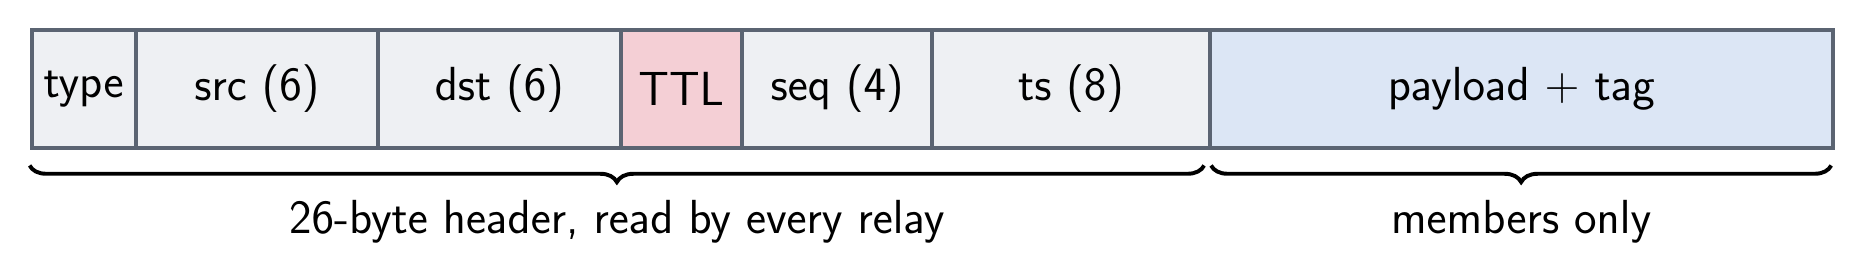
\begin{tikzpicture}[font=\fontsize{19}{23}\selectfont, x=2.2mm, y=1mm,
  f/.style={draw=muted, line width=0.5mm, minimum height=15mm, inner sep=0pt, anchor=south west}]
  \foreach \x/\w/\t/\c in {0/6/type/hdr, 6/14/src (6)/hdr, 20/14/dst (6)/hdr,
                           34/7/TTL/accent!20, 41/11/seq (4)/hdr, 52/16/ts (8)/hdr}
    \node[f, fill=\c, minimum width=\w*2.2mm] at (\x,0) {\t};
  \node[f, fill=scr, minimum width=36*2.2mm] at (68,0) {payload + tag};
  \draw[decorate, decoration={brace, amplitude=6pt, mirror}, line width=0.5mm] (0,-2) -- (67.8,-2)
    node[midway, below=3mm] {26-byte header, read by every relay};
  \draw[decorate, decoration={brace, amplitude=6pt, mirror}, line width=0.5mm] (68.2,-2) -- (104,-2)
    node[midway, below=3mm] {members only};
\end{tikzpicture}
\end{center}
\fig{Figure 2. Frame format; sizes in bytes. Duplicates are dropped on
(source, sequence).}

\sect{3\enspace Security}
\textbf{What each party learns.}\par
{\small
\begin{tabularx}{\linewidth}{@{}X>{\centering\arraybackslash}p{38mm}>{\centering\arraybackslash}p{38mm}>{\centering\arraybackslash}p{32mm}@{}}
\toprule
 & radio listener & relay, not a member & member \\
\midrule
addresses, hops left, time & yes & yes & yes \\
size and timing of traffic & yes & yes & yes \\
text of a group message & no & no & \textbf{yes} \\
forge or alter a message & no & no & yes \\
\bottomrule
\end{tabularx}}
\fig{Table 1. Payload privacy, not metadata privacy: the Bluetooth address
is stable and the header is in clear.}

\textbf{Group messages.} With $K_e$ the group key of epoch $e$, every
frame gets its own key, so a zero GCM nonce is never reused:
\begin{gather*}
K_{\mathrm{pkt}} = \mathrm{HKDF}(K_e;\ \mathit{src}\,\|\,\mathit{seq}\,\|\,\mathit{ts})\\
c = \mathrm{GCM}_{K_{\mathrm{pkt}}}(m;\ \mathit{header})
\end{gather*}
The header is authenticated as associated data, except TTL, which relays
decrement.


\sect{At the stand}
\fcolorbox{navy}{scr!45}{\begin{minipage}{0.95\linewidth}\vspace{3mm}
Three Thundercomm RUBIK Pi 3 screens (Qualcomm QCS6490) and three
Arduino UNO Q relays (Qualcomm QRB2210). Try it:
\begin{itemize}
  \item send from a screen: the message crosses a relay outside the group;
  \item exclude a board: it keeps relaying, and stops reading;
  \item restart the mesh: watch links and group come back.
\end{itemize}\vspace{3mm}
\end{minipage}}

\end{minipage}%
\hspace{20mm}%
% ================================================================ column 2
\begin{minipage}[t][935mm][t]{245mm}
\firstsect{Keys between members}
Each board $A$ holds an X25519
secret $a$ and an Ed25519 signing key. Every 30\,s it floods a signed
ANNOUNCE binding its address to $A = aG$. Two members then share a key
without ever having met:
\[ K_{AB}^{(e)} = \mathrm{HKDF}(aB,\ e) = \mathrm{HKDF}(bA,\ e) \]
since $aB = bA = abG$; nobody else can compute it.

\vfill
\begin{center}
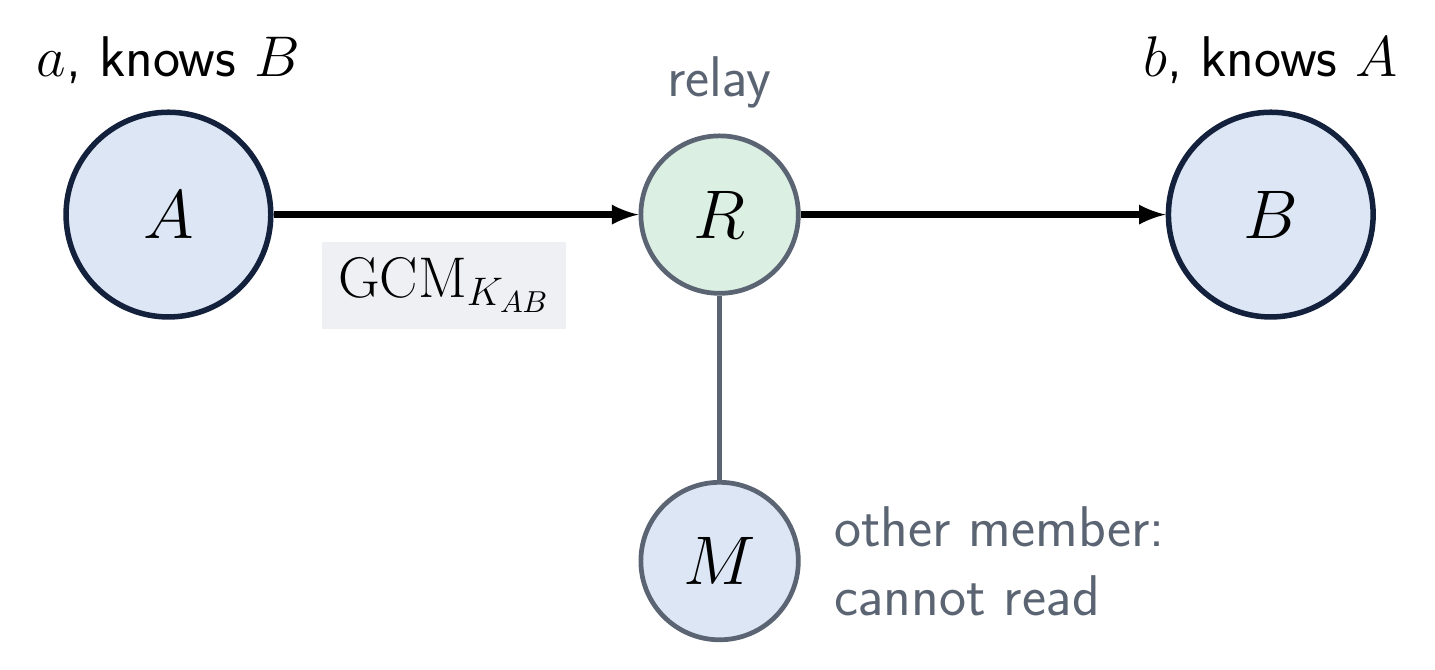
\begin{tikzpicture}[font=\small,
  m/.style={circle, draw=navy, line width=0.7mm, fill=scr, minimum size=26mm, inner sep=0pt},
  r/.style={circle, draw=muted, line width=0.6mm, fill=rel, minimum size=20mm, inner sep=0pt},
  o/.style={circle, draw=muted, line width=0.6mm, fill=scr, minimum size=20mm, inner sep=0pt}]
  \node[m] (a) at (0,0) {$A$};
  \node[r] (r) at (70mm,0) {$R$};
  \node[o] (c) at (70mm,-44mm) {$M$};
  \node[m] (b) at (140mm,0) {$B$};
  \draw[line width=0.8mm, -latex] (a) -- (r);
  \draw[line width=0.8mm, -latex] (r) -- (b);
  \draw[line width=0.6mm, muted] (r) -- (c);
  \node[above=2mm of a, font=\fontsize{21}{25}\selectfont] {$a$, knows $B$};
  \node[above=2mm of b, font=\fontsize{21}{25}\selectfont] {$b$, knows $A$};
  \node[above=2mm of r, font=\fontsize{21}{25}\selectfont, text=muted] {relay};
  \node[right=3mm of c, font=\fontsize{21}{25}\selectfont, text=muted, align=left] {other member:\\cannot read};
  \node[font=\fontsize{21}{25}\selectfont, fill=hdr, inner sep=2mm] at (35mm,-9mm) {$\mathrm{GCM}_{K_{AB}}$};
\end{tikzpicture}
\end{center}
\fig{Figure 3. A direct message from $A$ to $B$ crosses the mesh like any
frame, under a per-packet key derived from $K_{AB}$: relays and the other
members forward it but cannot read it.}

\vfill
\textbf{Removing a member $V$.} The coordinator $C$ (the member with the
smallest anonymous identifier) draws a new group key $K_{e+1}$ and a
one-time key $k$, and floods one frame. Each remaining member $i$ gets
$k$ wrapped under the pairwise key it shares with $C$:
\begin{gather*}
w_i = \mathrm{HKDF}(K_{Ci}^{(e)};\ \mathit{src}\,\|\,\mathit{seq}\,\|\,\mathit{ts})\\
\mathit{case}_i = \mathit{tag}_i \,\|\, \mathrm{GCM}_{w_i}(k) \qquad (i \neq V)\\
\mathit{body} = \mathrm{GCM}_k\big(e{+}1 \,\|\, K_{e+1} \,\|\, V \,\|\, \sigma_C\big)
\end{gather*}
where $\sigma_C$ is $C$'s Ed25519 signature over the epoch, the key and
the revoked key. There is no case for $V$.

\vfill
\begin{center}
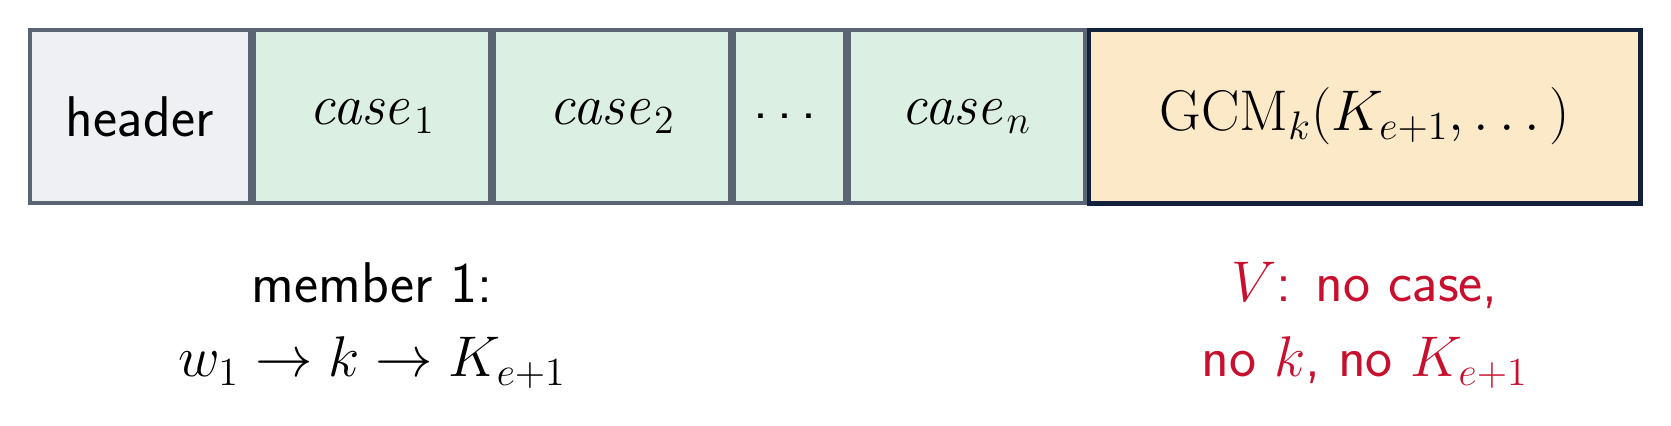
\begin{tikzpicture}[font=\fontsize{22}{27}\selectfont,
  c/.style={draw=muted, line width=0.5mm, minimum height=22mm, inner sep=1mm, fill=rel},
  h/.style={draw=muted, line width=0.5mm, minimum height=22mm, inner sep=1mm, fill=hdr},
  bd/.style={draw=navy, line width=0.6mm, minimum height=22mm, inner sep=1mm, fill=newk}]
  \node[h, minimum width=28mm, anchor=west] (hd) at (0,0) {header};
  \node[c, minimum width=30mm, right=0mm of hd] (c1) {$\mathit{case}_1$};
  \node[c, minimum width=30mm, right=0mm of c1] (c2) {$\mathit{case}_2$};
  \node[c, minimum width=14mm, right=0mm of c2] (cd) {\dots};
  \node[c, minimum width=30mm, right=0mm of cd] (cn) {$\mathit{case}_n$};
  \node[bd, minimum width=70mm, right=0mm of cn] (bo) {$\mathrm{GCM}_k(K_{e+1},\dots)$};
  \node[below=6mm of c1, align=center] (m1) {member 1:\\$w_1 \to k \to K_{e+1}$};
  \node[below=6mm of bo, align=center, text=accent] (v) {$V$: no case,\\no $k$, no $K_{e+1}$};
\end{tikzpicture}
\end{center}
\fig{Figure 4. The rekey frame. Relays, $V$ included, forward it
unchanged; only listed members can open it. The number of cases is
visible on the air.}

\vfill
Each member checks the signature, that the signer is the coordinator,
and that the epoch increases, then switches to $K_{e+1}$. $V$ keeps
relaying the new traffic but cannot read it. A newcomer can be excluded
only once its keys have been announced: wait one ANNOUNCE period after
a join.

\vfill
\textbf{What we accept in this prototype.}\par
{\small
\begin{tabularx}{\linewidth}{@{}>{\raggedright\arraybackslash}p{60mm}>{\raggedright\arraybackslash}X@{}}
\toprule
Who & What it can still do \\
\midrule
Non-member relay & drop or delay frames, rewrite TTL. \\
Active outsider & flood junk; pre-empt a (source, sequence) pair in relay caches. \\
Rogue member & grind its identifier to become coordinator. \\
Observer of a rekey & count the remaining members. \\
\bottomrule
\end{tabularx}}
\fig{Table 2. Availability attacks remain; the confidentiality and
authenticity of the payload do not depend on any relay.}

\vfill
\textbf{Checked.} On the boards, an excluded screen did not display the
next message (2 trials of 2). In simulation, from 6 to 30 nodes, no
remaining member was stranded and nothing leaked to the excluded one.
\end{minipage}%
\hspace{20mm}%
% ================================================================ column 3
\begin{minipage}[t][935mm][t]{245mm}
\firstsect{4\enspace Four hops across a building}
The stand fits on a table. Spread through the building, about 15\,m
apart with one relay off, the boards formed a line by themselves.

\vspace{6mm}
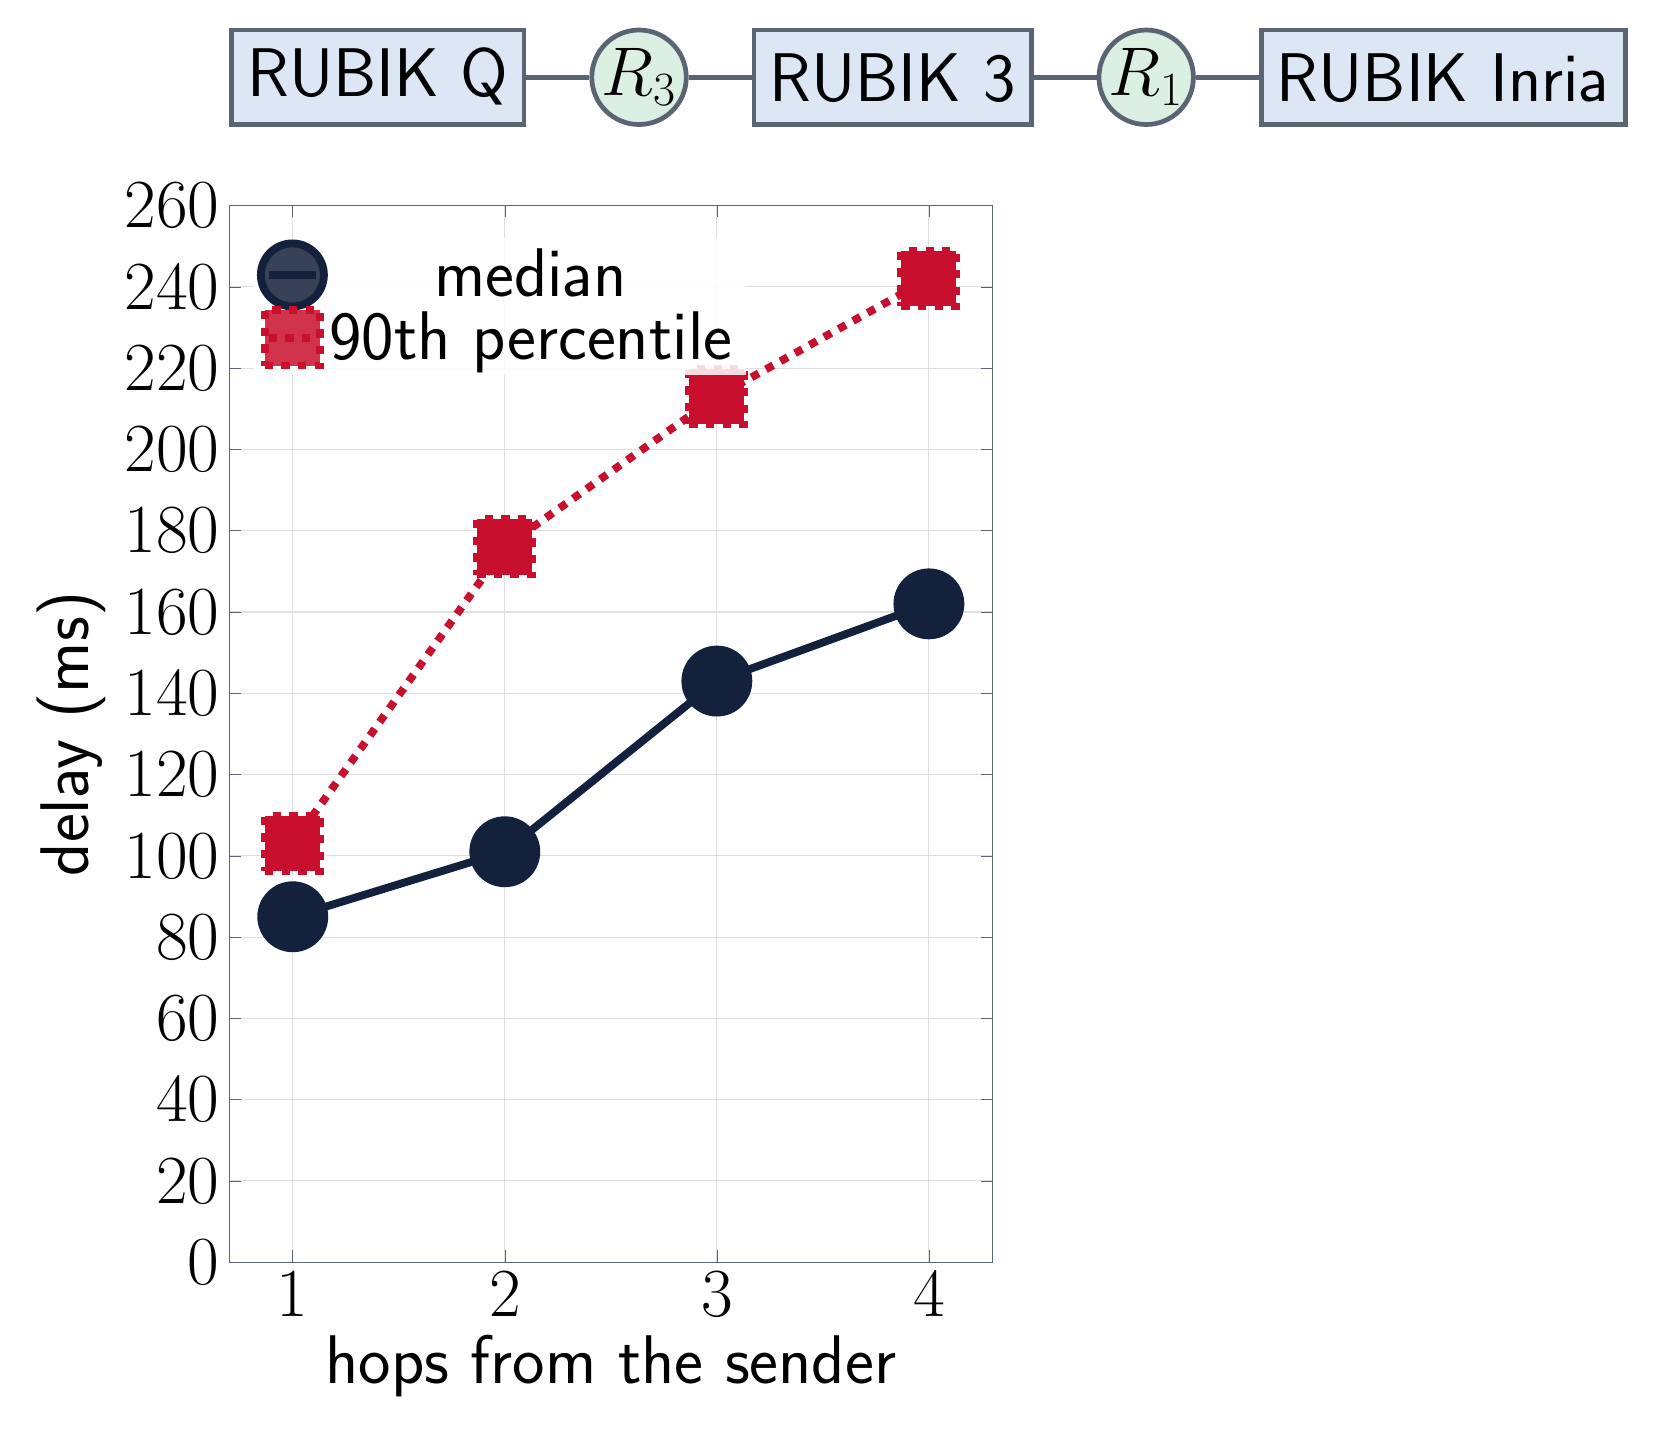
\begin{tikzpicture}[
  s/.style={draw=muted, line width=0.6mm, fill=scr, minimum height=12mm, inner sep=2mm, font=\small},
  r/.style={draw=muted, line width=0.6mm, circle, fill=rel, minimum size=12mm, inner sep=0pt, font=\small}]
\begin{axis}[height=150mm, xlabel={hops from the sender}, ylabel={delay (ms)},
  xmin=0.7, xmax=4.3, ymin=0, ymax=260, xtick={1,2,3,4}, legend pos=north west]
\addplot[line width=1mm, mark=*, mark size=4mm, navy] coordinates {(1,85) (2,101) (3,143) (4,162)};
\addlegendentry{median}
\addplot[line width=1mm, dashed, mark=square*, mark size=3.5mm, accent] coordinates {(1,103) (2,176) (3,213) (4,242)};
\addlegendentry{90th percentile}
\end{axis}
\node[s, anchor=south west] (a) at ([yshift=10mm]current axis.north west) {RUBIK Q};
\node[r, right=8mm of a] (b) {$R_3$};
\node[s, right=8mm of b] (c) {RUBIK 3};
\node[r, right=8mm of c] (d) {$R_1$};
\node[s, right=8mm of d] (e) {RUBIK Inria};
\foreach \u/\v in {a/b,b/c,c/d,d/e} \draw[line width=0.6mm, muted] (\u)--(\v);
\end{tikzpicture}
\fig{Figure 5. Send-to-display delay, on-board clocks within 50\,ms. The far
end received 76 of 79 messages, missing only those sent while the line
formed. Carried away, its link held to about 30\,m.}

\sect{5\enspace 8.2 hours on battery}
The stand on battery, one message every 30\,s: 988 messages, 4\,915
expected receptions.

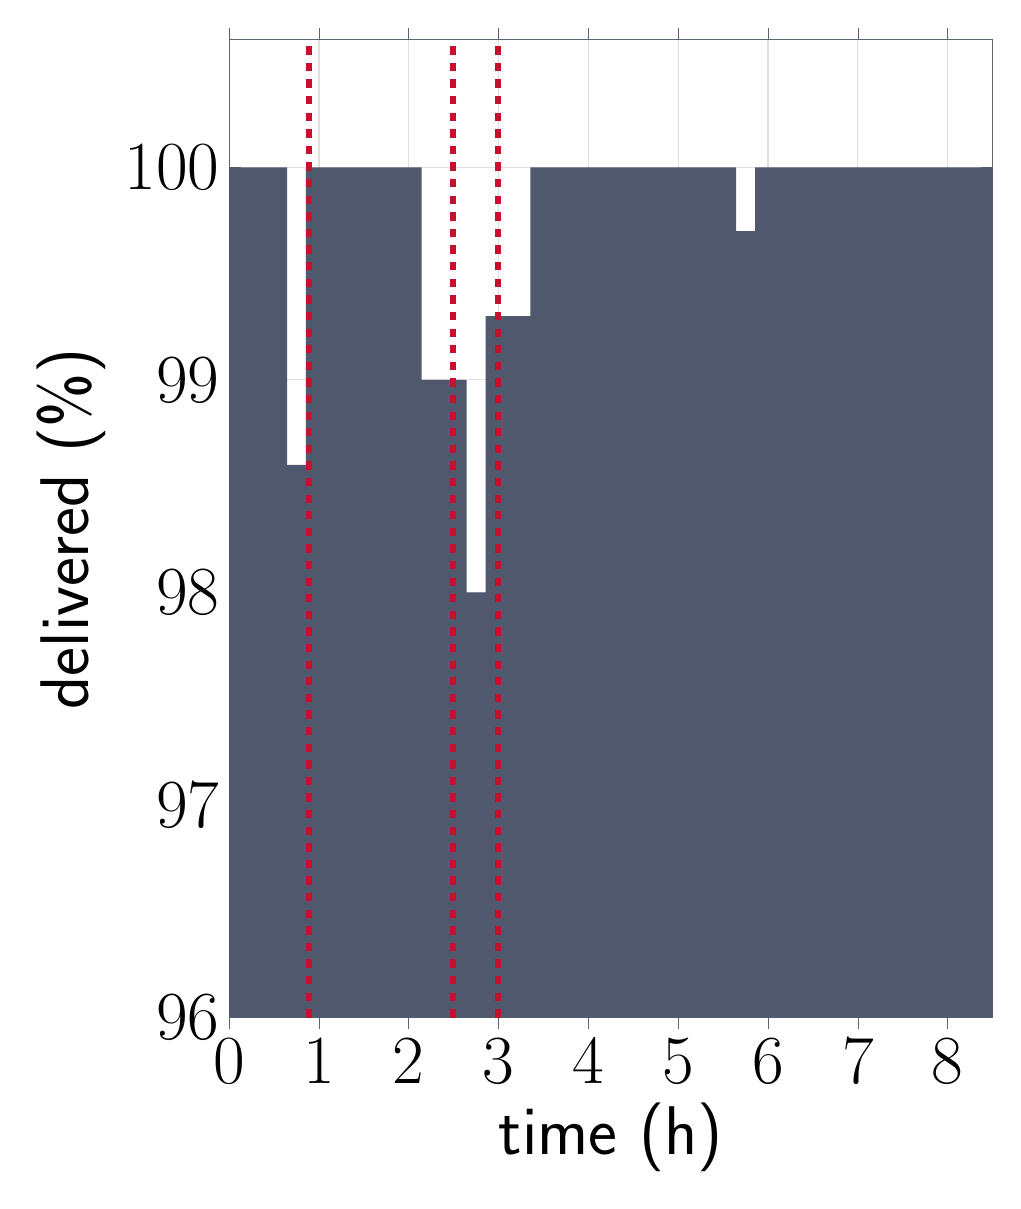
\begin{tikzpicture}
\begin{axis}[height=140mm, xlabel={time (h)}, ylabel={delivered (\%)},
  xmin=0, xmax=8.5, ymin=96, ymax=100.6, xtick={0,1,...,8}, ytick={96,97,98,99,100},
  ybar, bar width=9mm, bar shift=0pt]
\addplot[fill=navy!75, draw=none] coordinates {(0.25,100) (0.75,98.6) (1.25,100) (1.75,100)
  (2.25,99.0) (2.75,98.0) (3.25,99.3) (3.75,100) (4.25,100) (4.75,100) (5.25,100) (5.75,99.7)
  (6.25,100) (6.75,100) (7.25,100) (7.75,100) (8.12,100)};
\draw[accent, line width=0.8mm, dashed] (axis cs:0.89,96) -- (axis cs:0.89,100.6);
\draw[accent, line width=0.8mm, dashed] (axis cs:2.49,96) -- (axis cs:2.49,100.6);
\draw[accent, line width=0.8mm, dashed] (axis cs:2.99,96) -- (axis cs:2.99,100.6);
\end{axis}
\end{tikzpicture}
\fig{Figure 6. Delivery per 30 minutes. Dashed: a relay's Bluetooth
controller stopped answering and was reloaded without a reboot. Screens
received 100\,\%, relays 99.3\,\%; median delay 80\,ms, 99th percentile
188\,ms; 6 of 6 boards still up when stopped.}

\sect{6\enspace Limits and next steps}
\begin{itemize}
  \item A restarted sender restarts its sequence numbers, which the
        receivers' anti-replay windows reject: they must survive a
        restart.
  \item Two earlier defects, also found by measuring, are fixed with
        regression tests: ANNOUNCE and data shared one anti-replay
        window, and a sparse mesh could elect several coordinators.
  \item TTL\,10 spans about twenty nodes in simulation; on a line, one
        relay is a single point of failure.
  \item Next: an Android port, and replaying the protocol on the contact
        graph the link logs already record, to see how election and
        revocation behave when people move.
\end{itemize}

\vspace{6mm}
{\fontsize{16}{20}\selectfont\color{muted}
[1] N. Achir, P. Jacquet, BUBBLE-BLUE, arXiv:2509.00967, 2025.
[2] Bluetooth SIG, Mesh Profile 1.0, 2017.
[3] J. Dorsey et al., BitChat, 2025.
[4] M. R. Albrecht et al., Breaking Bridgefy, CT-RSA 2021.
[7] J. Wu, H. Li, connected dominating sets, DIAL-M 1999.
Boards provided by the Qualcomm University Platforms program.\par}
\end{minipage}
\end{document}
